\documentclass[tikz,border=8pt]{standalone}
% Shared look for every TikZ diagram. Load with \input{../../tools/tikz-style.tex}
\usepackage[T1]{fontenc}
\usepackage{lmodern}
\renewcommand{\sfdefault}{lmr}  % diagrams use the same serif as the text
\usetikzlibrary{arrows.meta, positioning, shapes.geometric, calc, fit, backgrounds}
\definecolor{cblue}{HTML}{4C78A8}
\definecolor{corange}{HTML}{F58518}
\definecolor{cgreen}{HTML}{54A24B}
\definecolor{cred}{HTML}{E45756}
\definecolor{cpurple}{HTML}{B279A2}
\definecolor{cgrey}{HTML}{6B6B6B}
\tikzset{
  every picture/.style={font=\sffamily, line width=1.2pt},
  box/.style={draw=#1, fill=#1!12, rounded corners=4pt, align=center, inner sep=7pt, minimum height=1.1cm},
  box/.default=cgrey,
  arrow/.style={-{Stealth[length=3mm]}, draw=cgrey, line width=1.4pt},
  title/.style={font=\sffamily\bfseries\Large},
  note/.style={font=\sffamily\small, text=cgrey, align=center},
}
\AtBeginDocument{\hyphenpenalty=10000 \exhyphenpenalty=10000}

\begin{document}
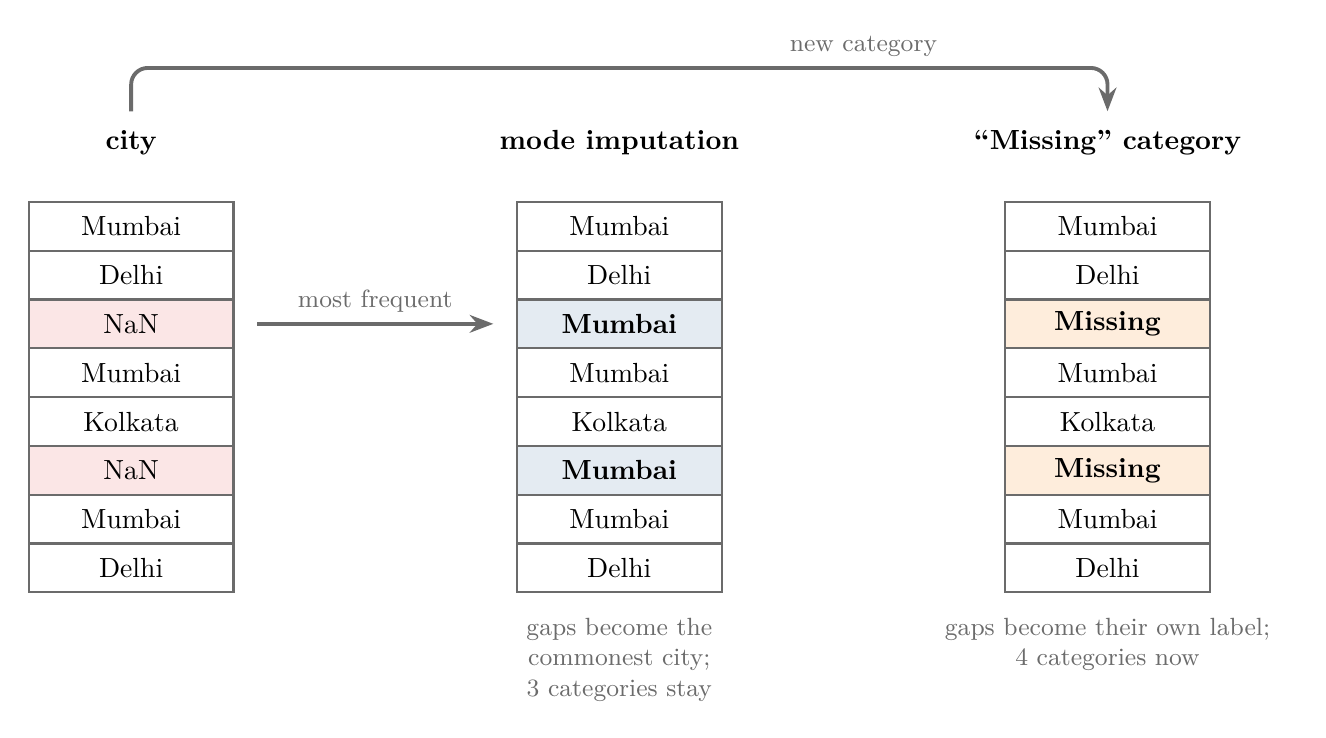
\begin{tikzpicture}
  % one small column with gaps, filled two ways
  \newcommand{\col}[4]{% #1 x, #2 title, #3 colour, #4 list of cells (text/colour)
    \node[font=\sffamily\bfseries] at (#1,0.75) {#2};
    \foreach \t/\c [count=\i] in {#4} {
      \node[draw=cgrey, fill=\c!15, minimum width=2.6cm, minimum height=0.62cm, line width=0.8pt]
        at (#1,-\i*0.62+0.31) {\t};
    }
  }
  \col{0}{city}{cblue}{Mumbai/white, Delhi/white, NaN/cred, Mumbai/white, Kolkata/white, NaN/cred, Mumbai/white, Delhi/white}
  \col{6.2}{mode imputation}{cblue}{Mumbai/white, Delhi/white, \textbf{Mumbai}/cblue, Mumbai/white, Kolkata/white, \textbf{Mumbai}/cblue, Mumbai/white, Delhi/white}
  \col{12.4}{``Missing'' category}{cblue}{Mumbai/white, Delhi/white, \textbf{Missing}/corange, Mumbai/white, Kolkata/white, \textbf{Missing}/corange, Mumbai/white, Delhi/white}
  \draw[arrow] (1.6,-1.55) -- node[above, font=\sffamily\small, text=cgrey] {most frequent} (4.6,-1.55);
  \draw[arrow, rounded corners=6pt] (0,1.15) -- (0,1.7) -- node[above, font=\sffamily\small, text=cgrey, pos=0.75] {new category} (12.4,1.7) -- (12.4,1.15);
  \node[note, text width=4.6cm, anchor=north] at (6.2,-5.15) {gaps become the commonest city;\\ 3 categories stay};
  \node[note, text width=4.6cm, anchor=north] at (12.4,-5.15) {gaps become their own label;\\ 4 categories now};
\end{tikzpicture}
\end{document}
